\section{Projekt robota}
\subsection{Założenia projektowe}
Wykonany robot powinien być jak najmniejszy i najprostszy w wykonaniu oraz sterowaniu tak aby móc przetestować przy jego pomocy działanie algorytmu A*. 
Robot będzie zbudowany z platformy, do której zostaną przyczepione napędy, elektronika sterująca oraz bateria. 
Do platformy zostaną przymocowane dwa gotowe moduły napędowe składające się z silnika, przekładni oraz dużego koła. 
Aby pojazd stał stabilnie, doczepione zostanie trzecie koło obracające się swobodnie w każdym kierunku.
Całość będzie sterowana przy pomocy mikroprocesora ESP32 oraz dwukanałowego sterownika silników DC opartym na układzie L298n.
Za zasilanie będzie odpowiadał litowo-jonowy akumulator 4S.

\subsection{Projektowanie zarysu robota w środowisku CAD}
Robot ma być prosty w budowie i wykonaniu, a więc założyłem, że podstawa utrzymujące pozostałe komponenty
zostanie wydrukowana na drukarce 3D. Model platformy i pozostałych posiadanych elementów został wykonany w programie Fusion 360.
Modele modułów napędowych, przedniego kółka oraz baterii pozwoliły na optymalne wyznaczenie pod względem wielkości lokalizacji wszystkich elementów.

% TODO: uprościć schematy z kicada

\begin{figure}[H]
	\centering
	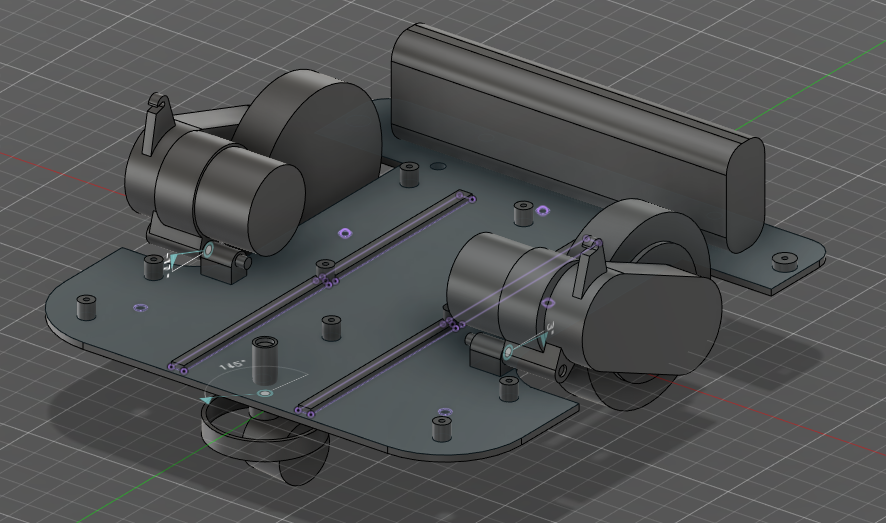
\includegraphics[width=10cm]{pages/robot/zdjecia/robotModelCaly.png}
	\caption{Zaprojektowane podwozie robota w programie Fusion360}
	\label{fig:Rys}
\end{figure}

\begin{figure}[H]
	\centering
	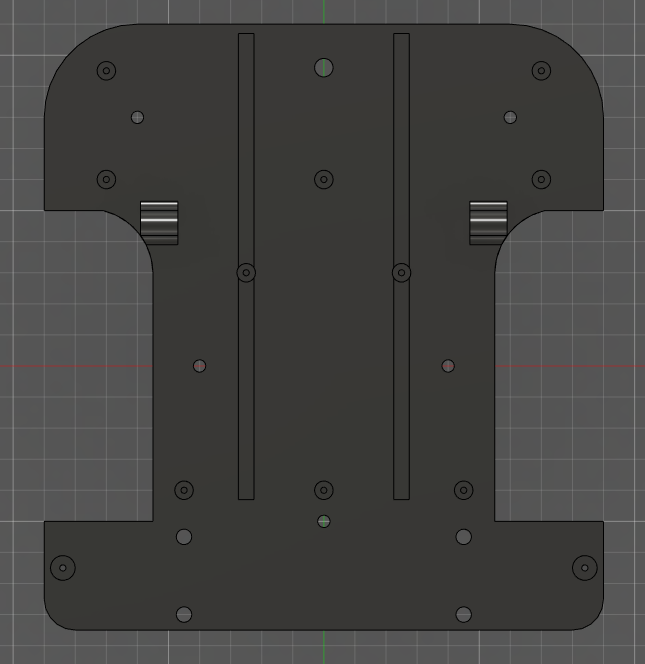
\includegraphics[width=10cm]{pages/robot/zdjecia/robotModelRama.png}
	\caption{Widok z góry na podwozie robota}
	\label{Fig:Rysunek}
\end{figure}
Model został przygotowany do druku w programie Ultimaker Cura a parametry druku zostały dobrane 
eksperymentalnie. Podstawę wydrukowano z PLA w temperaturze 220*C i wysokości warstwy 0,2mm. 
Żeby zwiększyć wytrzymałość temperatura głowicy została lekko zawyżona względem wymagań producenta filamentu.
\begin{figure}[H]
	\centering
	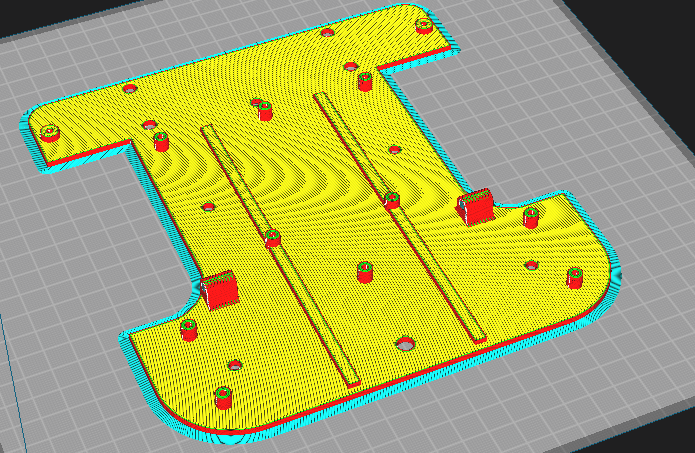
\includegraphics[width=13cm]{pages/robot/zdjecia/robotRamaCura.png}
	\caption{Widok przygotowanego do druku modelu}
	\label{fig:Rysunek}
\end{figure}
\subsection{Projekt, wykonanie oraz podłączenie elektroniki robota}
Ze względu na chęć bezprzewodowego sterowania robotem zostanie wykorzystany moduł ESP32, dla którego zostanie przygotowana odpowiednia płytka 
z wyprowadzeniami do enkoderów silnika oraz ich sterownika. Schemat elektroniczny i projekt pcb został wykonany w programie KiCad. 
\begin{figure}[H]
	\centering
	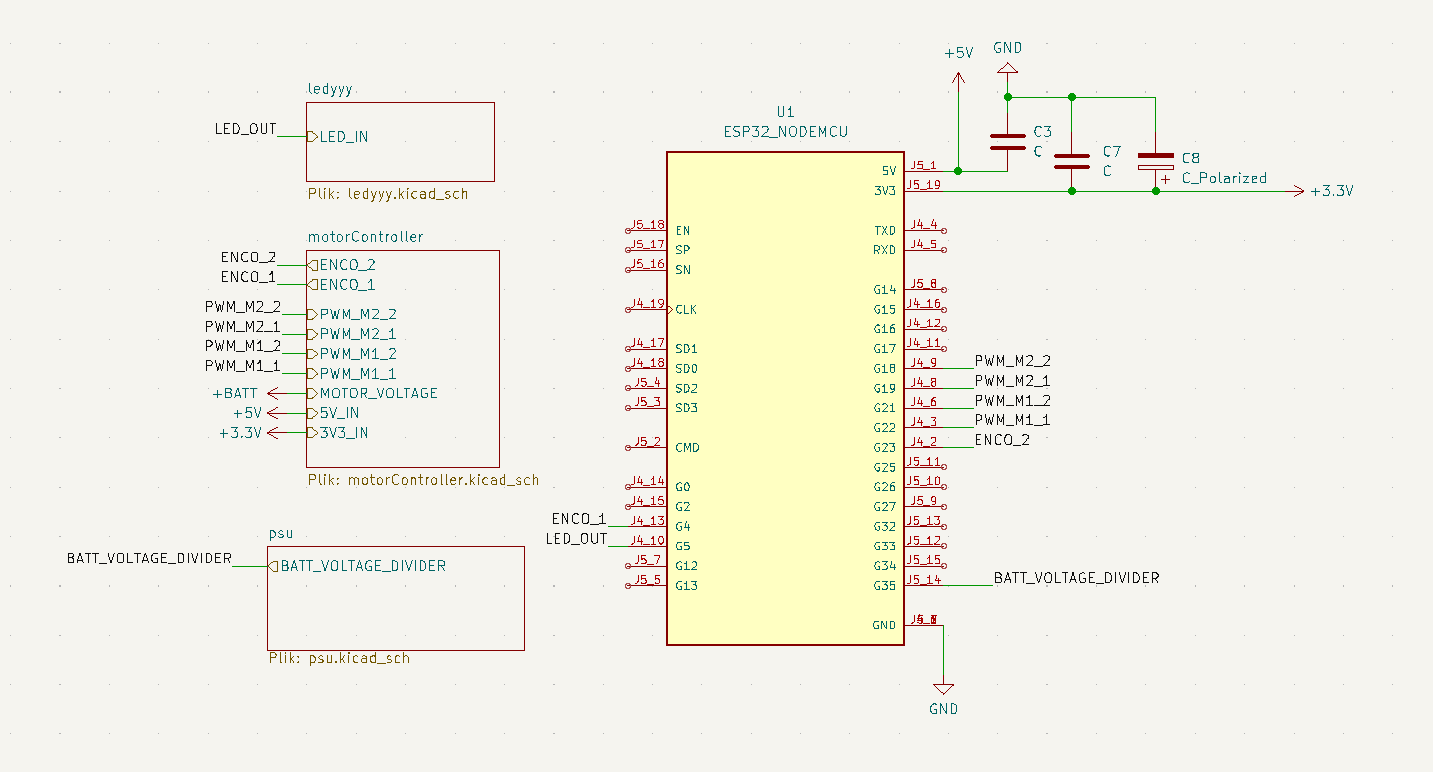
\includegraphics[width=13cm]{pages/robot/zdjecia/kicad/schematCaly.png}
	\caption{Ogólny schemat połączeń}
	\label{Fig:Rysunek}
\end{figure}
Wszystkie potrzebne elementy podsystemów mikroprocesora zostały już wlutowane w module deweloperskim,
a więc mój schemat zawiera jedynie odpowiednie połączenia z modułami roboczymi.
\begin{figure}[H]
	\centering
	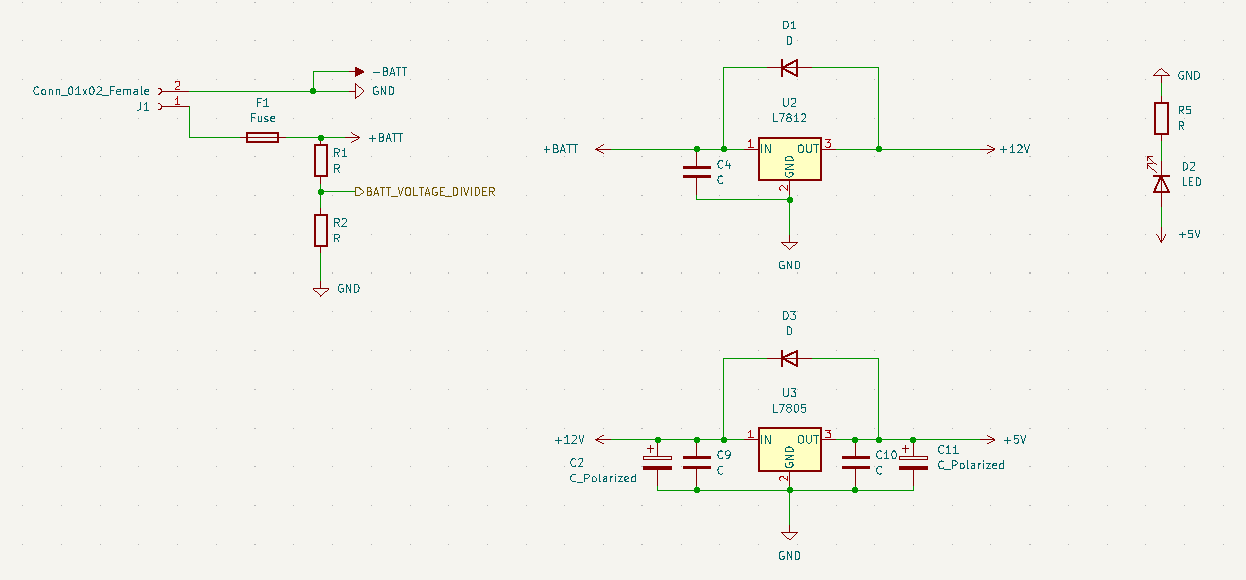
\includegraphics[width=10cm]{pages/robot/zdjecia/kicad/schematZasilanie.png}
	\caption{Ogólny schemat połączeń}
	\label{Fig:Rysunek}
\end{figure}
Użyta bateria posiada napięcie maksymalne 16,8V a więc musi zostać odpowiednio zmniejszone przed podaniem go na piny zasilania. 
Ze względu na wykorzystywaną łączność bezprzewodową a więc zwiększone zużycie prądu, zmniejszanie napięcia zostało podzielone na trzy sekcje. 
Najpierw zmniejszane jest poprzez stabilizator LM7812 z 16.8V do 12V, a następnie poprzez LM7805 z 12V napięcie redukowane jest do 5V. 
ESP32 zasilane jest napięciem 3.3V tworzonym poprzez stabilizator AMS1117 w module deweloperskim. 
Aby zredukować spadki napięć powstałe przy nagłym poborze prądu dodałem dodatkowe kondensatory filtrujące. 
Dodatkowo na schemacie widoczny jest dzielnik napięcia pozwalający na poziom naładowania baterii przez sterownik oraz programowalne diody świecące ws2812b,
jednak ostatecznie nie zostały wykorzystane w projekcie.
\begin{figure}[H]
	\centering
	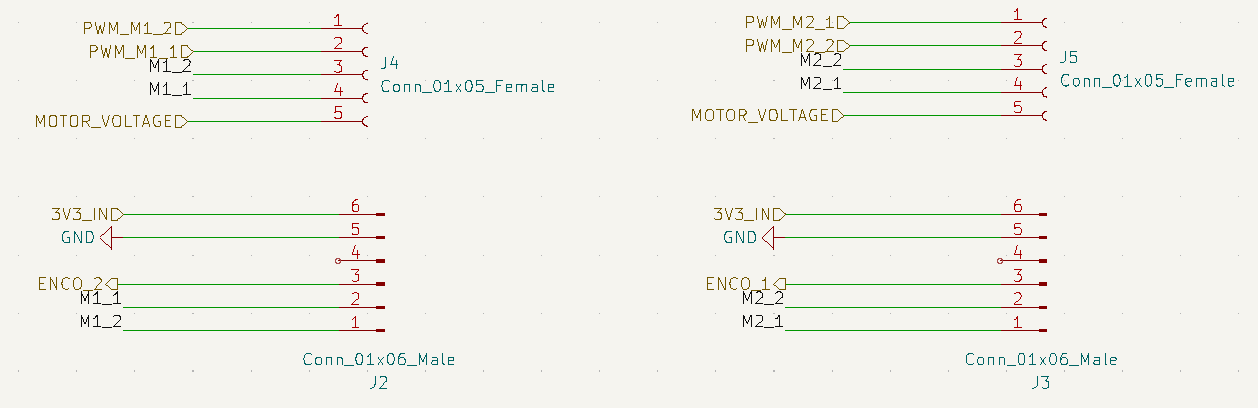
\includegraphics[width=16cm]{pages/robot/zdjecia/kicad/schematSilniki.png}
	\caption{Ogólny schemat połączeń silników}
	\label{Fig:Rysunek}
\end{figure}
Użyte moduły napędowe posiadają enkoder inkrementalny zbudowany z czujnika halla i tarczy magnetycznej zamocowanej na wale silnika.
Czujnik halla jest zasilany napięciem 3.3V i na wyjściu otrzymujemy sygnał ze "szpilkami" proporcjonalny do aktualnych obrotów silnika. 
Silniki zasilane są poprzez moduł z układem L298n, a prędkość ustalana jest poprzez odpowiednio generowany sygnał PWM. 
\begin{figure}[H]
	\centering
	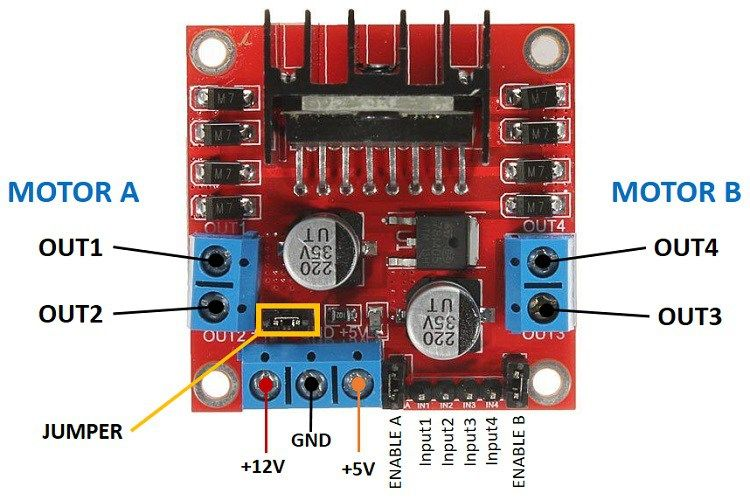
\includegraphics[width=10cm]{pages/robot/zdjecia/l298n_modul.jpg}
	\caption{Wykorzystany moduł do sterowania silnikami, L298n}
	\label{Fig:Rysunek}
\end{figure}
\begin{figure}[H]
	\centering
	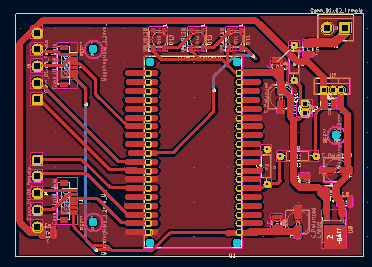
\includegraphics[width=6cm]{pages/robot/zdjecia/kicad/kiCad_PCB.png}
	\caption{Projekt PCB}
	\label{Fig:Rysunek}
\end{figure}
Na widocznym powyżej zdjęciu widać ostateczną wersje projektu pcb.


\subsection{Oprogramowanie robota}

Program sterujący robotem został napisany w C++. 
Szkielet aplikacji bazuje na projekcie utworzonym przez framework IDF w wersji 4.4 udostępnionym 
przez producenta użytego procesora. Po za tym użyta została biblioteka implementująca 
system czasu rzeczywistego FreeRTOS i ASIO do obsługi połączenia TCP. 
\begin{figure}[H]
	\centering
	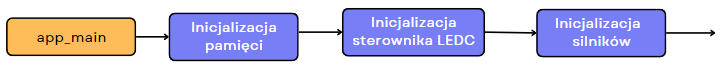
\includegraphics[width=14cm]{pages/robot/zdjecia/schematy/softSchematCz1.png}
	\caption{Schemat programu cz.1 }
	\label{Fig:Rysunek}
\end{figure}
\begin{figure}[H]
	\centering
	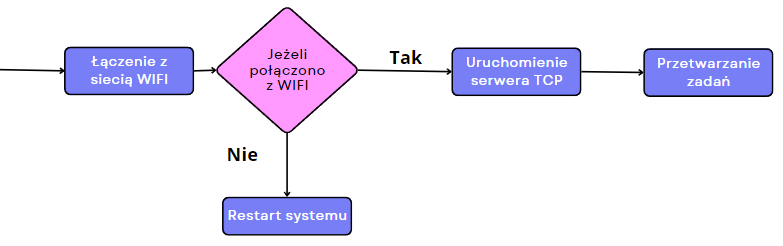
\includegraphics[width=14cm]{pages/robot/zdjecia/schematy/softSchematCz2.png}
	\caption{Schemat programu cz.2}
	\label{Fig:Rysunek}
\end{figure}

Działanie programu rozpoczyna się od wywołania funkcji app\_main, inicjalizacji funkcji systemowych i sterowników silników.
W dalszej kolejności nawiązywana jest łączność z siecią WiFi. W przypadku braku połączenia system resetuje się. 
Po poprawnym połączeniu uruchamiany jest kontekst biblioteki ASIO, a następnie uruchomienie serwera TCP.
Klienci po połączeniu do utworzonego serwera wysyłają komendy tekstowe wraz z odpowiednimi argumentami, które
robot odpowiednio przetwarza. 

\subsubsection{Sterowanie silnikami}
Sterowanie silnikami odbywa się poprzez klasę MotorController, która dziedziczy po klasie PIDController implementującej regulator PID.
Obiekt automatycznie tworzy timer uruchamiający co 100ms metodę aktualizującą wyjścia sterujące silnikiem. 
Aktualna prędkość wyznaczana jest na podstawie przerwania wyzwalanego przez enkoder silnika. Przerwanie inkrementuje licznik, 
czyszczony przez wcześniej opisany timer. Nastawy regulatora PID zostały dobrane eksperymentalnie, człon proporcjonalny wynosi 8 a całkujący i różniczkujący 0,1. 
Regulator PID możemy opisać przy pomocy wzoru:

\begin{equation}
	u(x) = e(x) * P + \int{e(x)} * I + \partial{e(x)} * D 
	\label{Eq:PID}
\end{equation}
Gdzie: $e(x)$ -- jest błędem; P,I,D -- to stałe odpowiednio członu proporcjonalnego, całkującego i różniczkującego

\begin{equation}
	e(x) = y_nast(x) - y_aktu(x)
	\label{Eq:blad}
\end{equation}
Gdzie: $y_nast(x)$ -- to nastawa regulatora, $y_aktu(x)$ -- jest rzeczywistą zmierzoną wartością
 
Powyżej przedstawiony regulator został zaimplementowany w funkcji calcOutput klasy PIDController.

\begin{lstlisting}[language=C++,caption=Zaimplementowany w C++ regulator PID,label={kodCPPPIDOutput}]
float PIDController::calcOutput(float current, float set)
{
	float error = set - current;
	float der = (error - this->_lastValue)/(_timeStep* 0.001);
	
	float output =  (this->_p * error) + 
					(this->_i * error * this->_timeStep * 0.001) + 
					(this->_d * der);

	this->_lastValue = error;
	return output;
}
\end{lstlisting}

Do wyznaczenia części różniczkującej potrzebna wartość błędu z poprzedniego wywołania pętli a ta zapisywana jest do zmiennej prywatnej klasy lastValue. 
Całkowanie zrealizowane jest poprzez pomnożenie przez krok dyskretyzacji. Stałe regulatora ustawiane są poprzez wywołanie konstruktora klasy.

Tak zaimplementowany regulator używany jest do wyznaczenia sygnału PWM, bezpośredniego sterującego układem L298n a ten silnikami. 

\begin{lstlisting}[language=C++,caption=Wyznaczenie modulacji PWM,label={kodCPPPWM}]
if(abs(setSpeed) - 1 > 0) // jezeli predkosc jest wieksza to pid jak nie to hamulec bo pwm=0
{
	pidToPwm = (int) this->calcOutput(abs(this->getCalculatedEngineRadialSpeed()), abs(setSpeed));
	if(setSpeed < 0)
	{
		pwmCh = 1;
	}
	else
		pwmCh = 0;

	pidToPwm += ledc_get_duty(LEDC_LOW_SPEED_MODE, this->_chanels[pwmCh]);
	pidToPwm = std::min(pidToPwm, 8192);
	pidToPwm = std::max(pidToPwm, 0);
}

// ustawienie wyjsc
ledc_set_duty(LEDC_LOW_SPEED_MODE, this->_chanels[pwmCh], (int)pidToPwm);
ledc_update_duty(LEDC_LOW_SPEED_MODE, this->_chanels[pwmCh]);

// ustawienie drugiego kanalu
ledc_set_duty(LEDC_LOW_SPEED_MODE, this->_chanels[(pwmCh==0)?1:0], 0);
ledc_update_duty(LEDC_LOW_SPEED_MODE, this->_chanels[(pwmCh==0)?1:0]);
\end{lstlisting}

W pierwszej kolejności sprawdzana jest zadana prędkość, jeżeli ta jest zbyt niska to na piny wystawiane są bezpośrednio stany niskie.
Jeżeli ustawiona prędkość jest poprawna to wyznaczamy wyjście regulatora. Sterowanie kierunkiem obrotów odbywa 
się poprzez znak zadanej prędkości a więc regulator otrzymuje wartości bezwzględne. 
Wyjście regulatora PID sumowane jest z aktualną nastawą. Wyjścia pwm skonfigurowane są w częstotliwości 5kHz i rozdzielczości 13bitów. 
Przed wysłanie nastaw do kontrolera pwm, te są obcinane do obsługiwanych zakresów (tj. 0 - 8192).

\subsubsection{Serwer TCP}

Po podłączeniu zasilania i uruchomieniu systemu robot oczekuje na polecenia wysłane do robota poprzez protokół internetowy TCP. Serwer został napisany w oparciu o bibliotekę ASIO, pozwalającą na asynchroniczną obsługę wejścia i wyjścia (w tym sieci).
\begin{figure}[H]
	\centering
	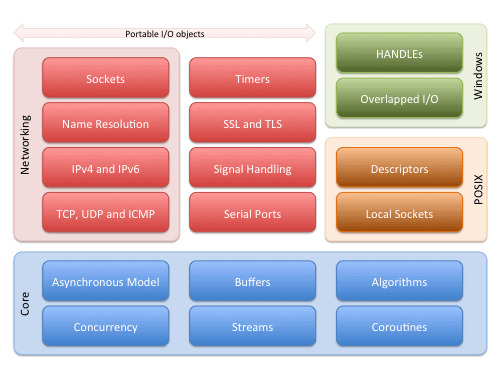
\includegraphics[width=10cm]{pages/robot/zdjecia/schematASIO.jpg}
	\caption{Schemat biblioteki ASIO \cite{asio}}
	\label{Fig:schematASIO}
\end{figure}
Biblioteka została napisana w C++ i pracuje w oparciu o standard POSIX wspierany również przez wykorzystywane ESP32.
Do akceptacji przychodzących połączeń została napisana klasa Server. Konstruktor przyjmuję referencje do kontekstu utworzonego w funkcji głównej programu. 
Uruchomienie kontekstu jest ważną częścią biblioteki ASIO, przetwarzane są w niej wszystkie asynchroniczne operacje.
Aby zapewnić jak najlepszy czas przetwarzania, kontekst uruchomiony jest w oddzielnym wątku przyłączonym do drugiego fizycznego rdzenia.

\begin{figure}[H]
	\centering
	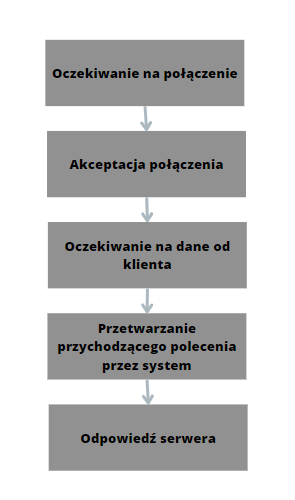
\includegraphics[width=6cm]{pages/robot/zdjecia/schematTCP.png}
	\caption{Schemat działania serwera TCP}
	\label{Fig:schematSerweraTCP}
\end{figure}

Po zaakceptowaniu przychodzącego połączenia, obiekt połączenia dodawany jest do specjalnej tablicy przechowującej wszystkich klientów. 
Dane mogą być równocześnie przetwarzane w kilku miejscach a więc używane są dzielone wskaźniki, które automatycznie usuwają dane jeżeli nikt z nich nie korzysta.
Na każdym aktywnym połączeniu prowadzony jest nasłuch, dzięki czemu możemy mieć równocześnie podłączony program do generowania ścieżki i drugi pozwalający na podgląd parametrów robota.
Klient wysyła polecenia w formie tekstowej, te przekazywane są do klasy systemowej odpowiednio interpretujące ich przeznaczenie.
Jeżeli komenda tego wymaga (np. zwrócenie prędkości obrotowej silników) to dane są odsyłane do klienta w postaci tekstu i oddzielonych przerwą liczb. 

% TODO: nawiązanie do serwera dhcp